\section{Case Study：医学影像 AI 问题拆解}
\label{sec:case}

\webref{docs/6-课题范式/}
\resref{resources/06-domain/}

\subsection{系统定位}
以医学影像辅助检测为例：临床痛点包括漏诊、微小/隐匿病灶与标准不一；系统能力可分层为提质增效（CADe）、智能预警与高级辅助。入门课题多落在阅片前自动检测与标记，且须明确辅助检出不等于替代诊断。

\subsection{问题画像与子问题框架}
技术上常同时面对小目标、异常检测与极度类别不平衡。推荐将 pipeline 正交拆为：弱信号保留、召回--假阳性权衡、多模态语义、工程部署、数据与标注、评价体系六类子问题。写作与开题时应先定义问题，再选择具体网络结构，避免手段与问题混淆。

\begin{figure}[htbp]
  \centering
  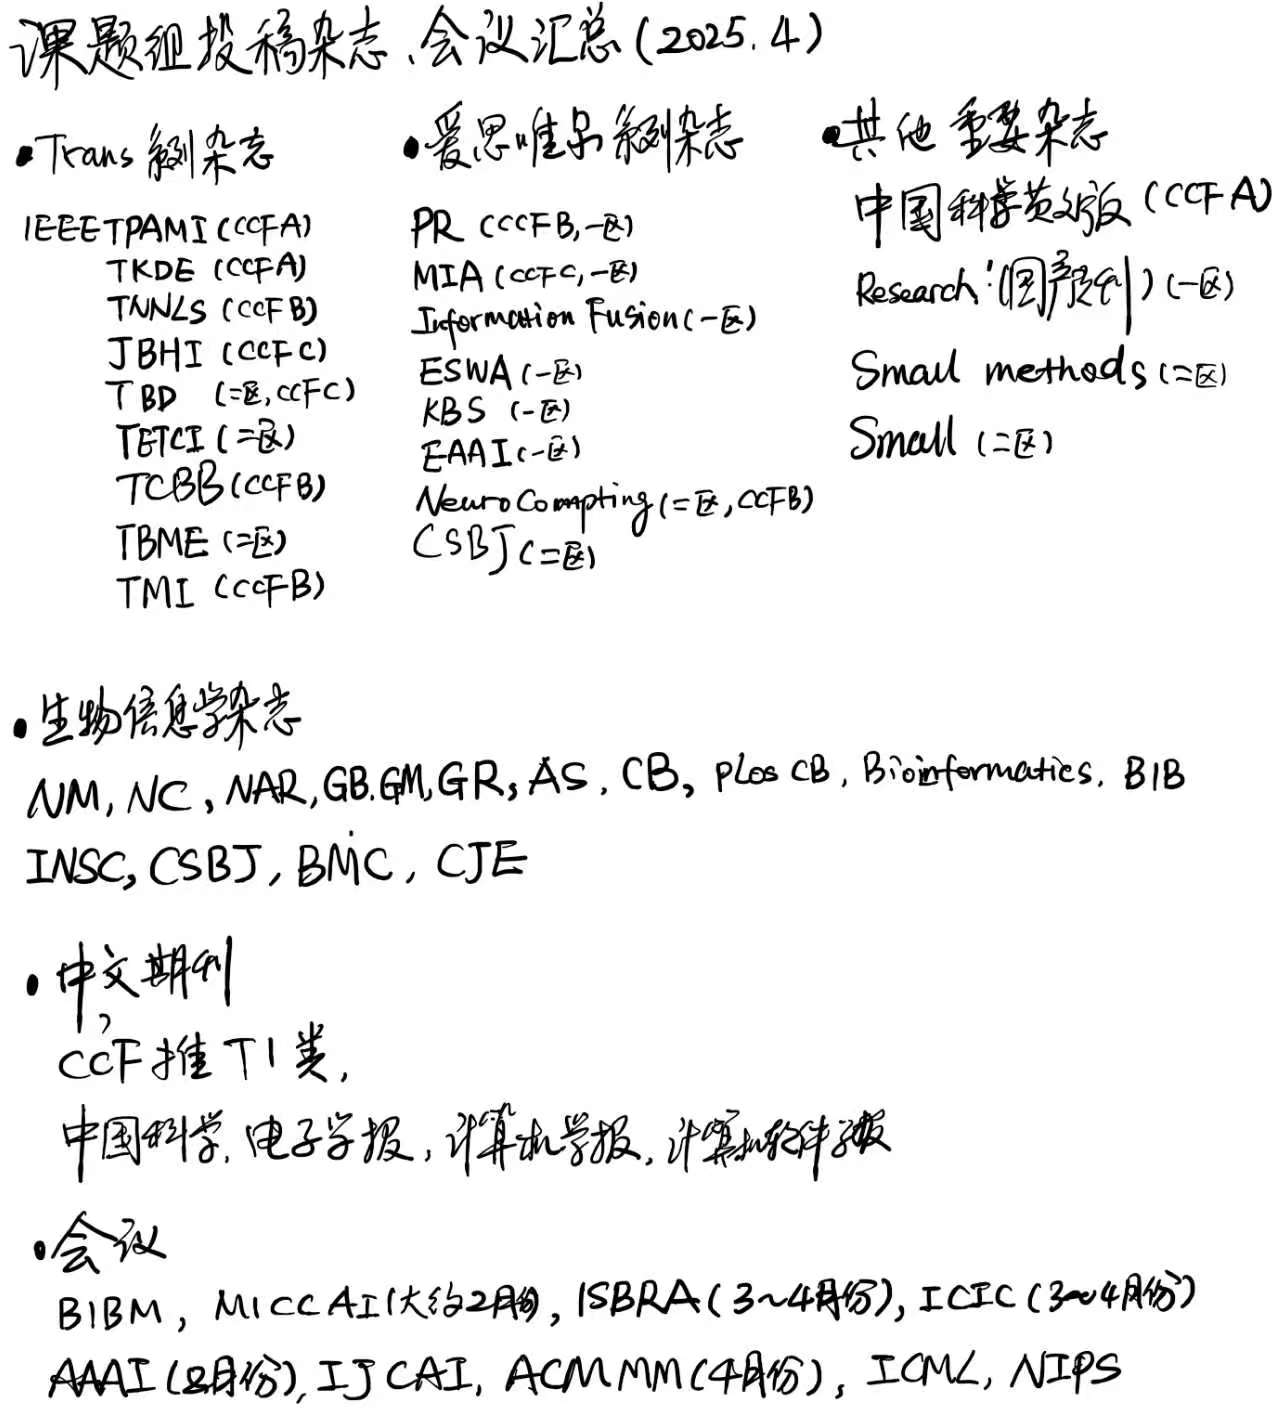
\includegraphics[width=0.9\textwidth]{figures/journal_list.jpg}
  \caption{课题组投稿期刊/会议汇总示意（以组内最新版为准）}
  \label{fig:journal-list}
\end{figure}

\subsection{数据与下一步}
数据集整理字段见 \path{resources/06-domain/dataset_sheet.csv}。公开入口包括 Nature Scientific Data、Grand Challenge、Kaggle 与 Papers with Code。四周内可针对 1--2 个子问题检索 SOTA、摸底数据许可、与导师确认成功标准，并完成文献 list 与一次短汇报。
